% 电生理结果
% - [ ] 能量谱提示主要的波段
% - [ ] 能量曲线的变化
% - [ ] 相位分析显示学习过程

\section{电生理记录与脑电频谱变化}
由于临床需要,医用不锈钢电极被放置在每位患者主要癫痫病灶区域,
用以监测和定位癫痫的起始位置。通过与华山医院的合作,以及患者
的同意,我们得以在患者进行行为学测试的同时,记录下相应电极的
电信号。癫痫多发于颞叶,而电极的主要记录位置因而集中在颞叶;
但其中有一例特别的病例,患者\#1的癫痫病灶集中在枕叶,因而得以
记录到来自视觉皮层的脑电信号(图\ref{fig:ephys_example}~a)。

\subsection{能量谱提示主要的波段}
首先,我们需要确定光栅刺激过后,脑电反应主要集中的频率范围。
我们对原始的数字信号(图\ref{fig:ephys_example}~b)进行了小波变化处理,并将每次光栅刺激的脑电信号
依据光栅开始的时间对齐,做出脑电信号频谱图(图\ref{fig:ephys_example}~c)。
通过频谱图可见,患者脑电的主要频谱集中在50至100赫兹,即\(\gamma\)波段(\(30 \sim 80\ \text{Hz}\))。
但在低频的区域,例如\(\delta\),\(\theta\)等波段,频谱图上能量的变化没有高频段那么明显,
与刺激时间的耦连性也没有\(\gamma\)波段那么广泛。

为了进一步量化脑电信号能量的变化,我们依据频谱获得的频率范围以及\(\gamma\)波段范围,选取了
相对应的50至80赫兹作为后续的探究范围。我们计算得到经过带通滤波的脑电信号的能量变化,
并以光栅刺激前的时间段作为基线,利用z-score归一化得到每个通道的能量曲线(图\ref{fig:ephys_example}~d)。
与能量频谱相同,能量曲线在光栅开始后也出现了明显的增强;同时,在光栅持续的时间段中,
能量曲线总体仍高于基线水平。

我们对小鼠的局部场电位信号也做了相同的分析处理(图\ref{fig:ephys_example}~e-g),
可以看到小鼠的频谱与患者的频谱相似,同样也涵盖了\(\gamma\)波段;
但相较而言小鼠的总体振荡比患者的稍偏低频一些。
而小鼠的能量曲线也同样在光栅开始后出现了明显的增强,并横跨了整个刺激期间。

局部场电位的能量变化,可以看作是局部脑区里所有神经元放电的强弱变化。
而小鼠和人的结果中,都提示了光栅的视觉刺激,可以引起视皮层脑区的放电;
同时,放电的频率主要集中在高频的\(\gamma\)波段。这也与过去的实验基本
保持一致\cite{lima2011gamma,demiralp2007gamma}。

\begin{figure}[h]
    \centering
    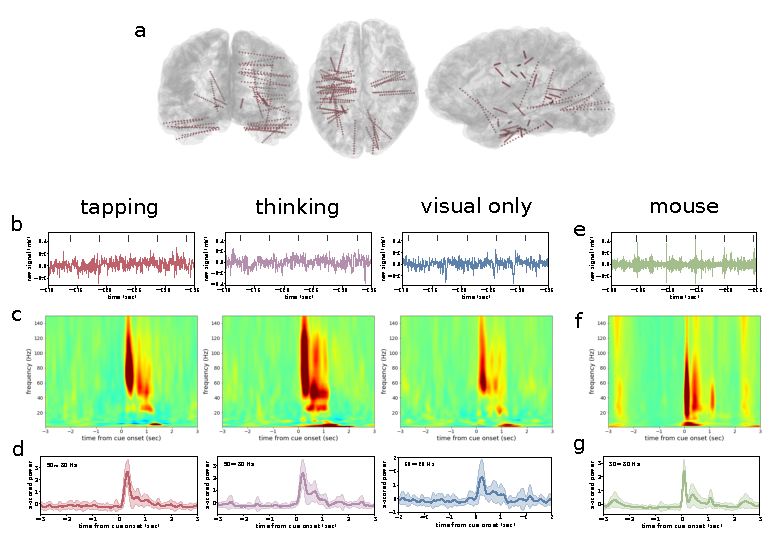
\includegraphics[width=\textwidth]{src/figures/ephys_examples.pdf}
    \caption{\textbf{电生理记录通道示例}\\
    (\textbf{a})~电极的脑区定位。每个红点均为一个记录通道,这里将记录到的
    6位患者的电极画在一起。(\textbf{b-d})~不同行为范式下
    同一个通道的示例。b: 脑电信号的原始形式,黑色的竖线对应光栅定时的时间。
    c: 脑电信号通过小波变化得到的能量频谱,展现了信号能量主要集中于\(\gamma\)波段。
    d: 带通滤波后的脑电信号能量曲线。
    (\textbf{e-g})~小鼠中局部场电位的示例。}
    \label{fig:ephys_example}
\end{figure}

\subsection{能量曲线的变化趋势}
依据患者的术前MRI和术后CT,我们得以对每个电极进行定位。
我们从患者\#1中选择了通道数目最多的三个脑区,
视觉皮层(visual cortex, 主要为Brodmann分区17、18、19, 共计32个通道),
扣带回(cingulate cortex, 主要为Brodmann分区30、31,共计18个通道),
以及颞中回(middle temporal gyrus, 主要为Brodmann分区21,共计10个通道)。

对相同脑区下的脑电能量曲线进行平均后(图\ref{fig:ephys_network}~a),
我们发现三个脑区的能量曲线形态十分相似,提示光栅视觉刺激可能会引起全脑范围的活动。
另一方面,对于三种不同的行为范式,轻拍手和默想下的能量曲线基本一直,而空想下的
能量曲线较前两者有明显的下降。%TODO statistical significance
提示注意力的集中程度可能会影响大脑的整体活动,但需要额外的实验进行验证和探究。

%扩散方向

\subsection{相位分析显示学习过程}
脑电信号可以被看作是一种特殊的数字信号,因而我们进一步计算了脑电信号的相位信息。
不同于信号的能量,相位的绝对值没有实际的生物学意义,但相位可以被认为
是一种神经元群体放电的状态\cite{gu2010phase}。
而相位和能量之间存在着一定的耦连关系\cite{watrous2015phase,demiralp2007gamma}
由于相位的变化通常体现在较低的频段,我们选取了\(\delta\)波段(\(0.5 \sim 4\ \text{Hz}\))作为相位分析的对象。
为了量化脑电信号的相位,我们将同一天中20次刺激下的脑电信号分为一组,
计算了各组的ITPC值,并对各个通道的ITPC值依照脑区进行平均(图\ref{fig:ephys_network}~b)。
可见,患者的脑电出现了两次相位锁定(phase locking),分别位于光栅开始和光栅结束。
其中,对于轻拍手和模型范式,ITPC值基本一致;
而空想下,ITPC值较前两者明显降低。%TODO statistical significance
提示在空想下的放电活动的一致性不如轻拍手和默想范式。

同时,我们也对小鼠的脑电信号做了相同的相位分析(图\ref{fig:ephys_network}~c)。
与患者的相位不同,小鼠的脑电只有在光栅开始后有一次相位锁定,而在光栅结束后没有。
由于小鼠每天进行的实验测试数量较大,因而小鼠相位的ITPC值更加趋向于真实值,即
基线更接近于0。而人的实验中,每种范式每个时间间隔只有20次刺激,存在一定的随机
因素,因而其基线更高;但总体的趋势不会发生变化。

此外,我们将轻拍手范式下,依据患者是否存在提前打手(即,是否能够较为准确的预判时间间隔),
将脑电信号分为两组,即提前打手组和延后打手组。我们对这两组的脑电信号分别计算了
各自的ITPC值(图\ref{fig:ephys_network}~d),发现延后打手的行为中,脑电信号的
相位没有出现提前打手下的相位锁定现象。提示能否准确预测时间间隔,
可能会造成相同视觉刺激下的不同放电模式。
% 为了进一步确认不同行为表现下相位确实存在差异,
% 我们对每个通道不同行为表现下的相位变化进行了主成分分析(图\ref{}~a)

\begin{figure}[h]
    \centering
    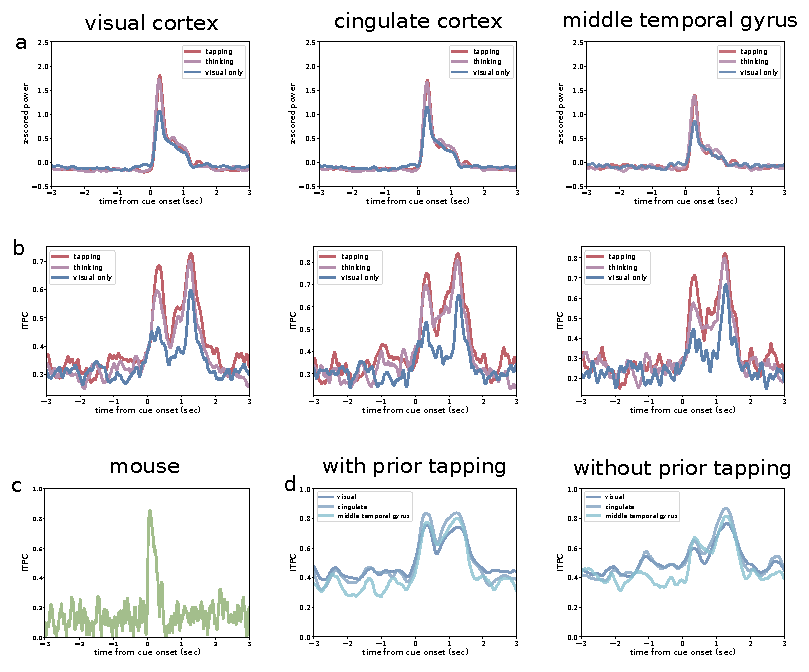
\includegraphics[width=\textwidth]{src/figures/ephys_network.pdf}
    \caption{\textbf{不同脑区下能量曲线与相位锁定}\\
    (\textbf{a})~不同脑区不同行为范式下的能量曲线。
    (\textbf{b})~不同脑区不同行为范式下的相位变化。
    (\textbf{c})~小鼠场电位的相位变化。
    (\textbf{d})~轻拍手范式下,提前打手(准确预判)和延后打手(错误预判)的相位变化。}
    \label{fig:ephys_network}
\end{figure}

